\documentclass{article}
\usepackage{amsmath}
\usepackage{hyperref}
\usepackage{tikz} 
\usetikzlibrary{decorations.pathreplacing}
\usepackage[a4paper]{geometry}
\usepackage{fancyhdr}
\pagestyle{fancy}
\lhead{Hall Effekt}
\rhead{September 2025}
\begin{document}
\section{Hall Effekt}
\begin{minipage}{\dimexpr\linewidth-6cm} 
Fließt Strom durch einen Leiter der Maßen $d$, $l$ und $b$, welcher in einem Magnetfeld ist, so sorgt die \hyperref[Lorentzkraft]{Lorentzkraft} dafür, dass die elektronen, abgelenkt werden. Ist das Magnetfeld so wie in der Zeichung ausgerichtet, heißt aus Blickrichtung des Magnetfeldes nach rechts bewegend, so werden diese nach unten abgelenkt. \newline
Weil nun auf der unteren Seite der Leiters mehr Elektronen sind, kommt es zu einer Spannug, der \emph{Hallspannung} $U_H$. Dabei gilt
\end{minipage} 
\hfill 
\begin{minipage}{6cm} 
 \center
 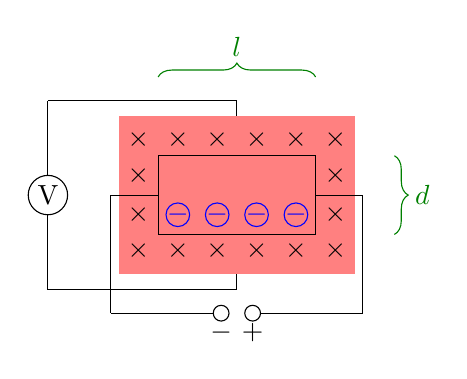
\begin{tikzpicture} 
  \fill[red!50] (-0.5, -0.5) rectangle (2.5, 1.5);
  \foreach \x in {-1,...,4} {
   \draw (0.25+0.5*\x, 1.2) node{$\times$};
   \draw (0.25+0.5*\x, -0.2) node{$\times$};
  };
  \foreach \x in {0, 1} {
   \draw (-0.25, 0.25+0.5*\x) node{$\times$};
   \draw (2.25, 0.25+0.5*\x) node{$\times$};
  };
  \foreach \x in {0,...,3} {
   \draw[blue] (0.25+0.5*\x, 0.25) circle (0.15cm) node{$-$};
  };
 
  \draw (0, 0) rectangle (2, 1);
 
  \draw (-0.6, 0.5) -- (0, 0.5);
  \draw (2, 0.5) -- (2.6, 0.5);
 
  \draw (-0.6, 0.5) -- (-0.6, -1);
  \draw (2.6, 0.5) -- (2.6, -1);
  \draw (-0.6, -1) -- (0.7, -1);
  \draw (1.3, -1) -- (2.6, -1);
  \draw (0.8, -1) circle (0.1cm) node[below] {$-$};
  \draw (1.2, -1) circle (0.1cm) node[below] {$+$};
 
  \draw (-1.4, 0.5) circle (0.25cm) node {V};   
  \draw (-1.4, 0.75) -- (-1.4, 1.7);
  \draw (-1.4, 0.25) -- (-1.4, -0.7);
  \draw (-1.4, 1.7) -- (1, 1.7);
  \draw (-1.4, -0.7) -- (1, -0.7);
  \draw (1, 1.7) -- (1, 1.5);
  \draw (1, -0.7) -- (1, -0.5);
 
  \draw [green!50!black, decorate,decoration={brace,amplitude=5pt,mirror}]
  (3,0) -- (3,1) node[midway,right,xshift=4pt]{$d$};
  \draw [green!50!black, decorate,decoration={brace,amplitude=5pt}]
  (0,2) -- (2,2) node[midway,above,yshift=4pt]{$l$};  
 \end{tikzpicture} 
\end{minipage}
 
\[
 U_H = \frac{1}{n \cdot e} \cdot \frac{B \cdot I}{d} 
\]
 
\subsection{Herleitung}%PROC Abiturrelevant
Auf die Elektronen wirken zwei Kräfte, die Lorentzkraft und die kraft des elektrischen Feldes 
\[
 F_L = B \cdot I \cdot L
 \qquad \text{und} \qquad
 F_{el} = Q \cdot E = e \cdot \frac{U_H}{d}
\] 
Die Stromstärke $I = \dfrac{Q}{t}$ eines einzelnen Elektrons nutzt als Ladung die Elektronenladung, also
\[
 F_L = B \cdot \frac{e}{t} \cdot l 
\]
Hier kann $\dfrac{l}{t}$ offensichtlich zu $v$, der Driftgeschwindigkeit des Elektrons innerhalb des Leiters, gekürzt werden. Somit gilt letztendlich die Lorentzkraft
\[
 F_L = B \cdot e \cdot v 
\] 
Solange eine auf ein Elektron wirkende Kraft stärker ist als die Andere, wird das Elektron ausgelenkt, also bewegt es sich bis beide Kräfte gleich stark sind.
\[
 e \cdot v \cdot B = e \cdot \frac{U_H}{d}
\]
Somit gilt
\[
 B = \frac{U_H}{v \cdot d} \implies U_H = B \cdot v \cdot d
\]
\end{document}